%\section{Используемые структуры}

%\captionsetup{singlelinecheck = false, justification=raggedright}
%\lstinputlisting[label=lst:author, caption=Фрагмент open.c, language=c]{structs/SYSCALL_DEFINE.txt}

%\captionsetup{singlelinecheck = false, justification=raggedright}
%\lstinputlisting[label=lst:author, caption=Фрагмент namei.c, language=c]{structs/namei.txt}

%\captionsetup{singlelinecheck = false, justification=raggedright}
%\lstinputlisting[label=lst:author, caption=Фрагмент file.c, language=c]{structs/file.txt}

%\captionsetup{singlelinecheck = false, justification=raggedright}
%\lstinputlisting[label=lst:author, caption=Фрагмент filename.h, language=c]{structs/filename.h}

%\captionsetup{singlelinecheck = false, justification=raggedright}
%\lstinputlisting[label=lst:date, caption=Фрагмент internal.h, language=c]{structs/openflags.h}

%\captionsetup{singlelinecheck = false, justification=raggedright}
%\lstinputlisting[label=lst:date, caption=Фрагмент audit.h, language=c]{structs/auditnames.h}

%\captionsetup{singlelinecheck = false, justification=raggedright}
%\lstinputlisting[label=lst:date, caption=Фрагмент namei.c, language=c]{structs/nameidata.h}

%\captionsetup{singlelinecheck = false, justification=raggedright}
%\lstinputlisting[label=lst:date, caption=Фрагмент openat2.h, language=c]{structs/openhow.h}

%\captionsetup{singlelinecheck = false, justification=raggedright}
%\lstinputlisting[label=lst:date, caption=Фрагмент open.c]{structs/build_open_how.txt}


\clearpage
\section*{Флаги системного вызова \texttt{open()}}

Версия ядра: \texttt{6.3.2}

\texttt{O\_APPEND} --- файл открывается в режиме добавления. Перед каждой
операцией записи файловый указатель будет устанавливаться в конец файла.

\texttt{O\_CREAT} --- если имя пути не существует, то файл создается как обычный файл.

\texttt{O\_EXCL} --- если используется совместно с \texttt{O\_CREAT}, то при
наличии уже созданного файла вызов завершится ошибкой.

\texttt{O\_NOCTTY} --- если файл указывает на терминальное устройство, то оно не
станет терминалом управления процесса, даже при его отсутствии.

\texttt{O\_TRUNC} --- если файл уже существует, он является обычным файлом и
заданный режим позволяет записывать в этот файл, то его длина будет урезана до
нуля.

\texttt{O\_NONBLOCK}, \texttt{O\_NDELAY} --- файл открывается, по возможности, в
режиме non-blocking, то есть никакие последующие операции над дескриптором файла
не заставляют в дальнейшем вызывающий процесс ждать.

\texttt{O\_SYNC} ---  файл открывается в режиме синхронного ввода-вывода, то
есть все операции записи для соответствующего дескриптора файла блокируют
вызывающий процесс до тех пор, пока данные не будут физически записаны

\texttt{O\_NOFOLLOW} --- если файл является символической ссылкой, то open
вернёт ошибку.

\texttt{O\_DIRECTORY} --- если файл не является каталогом, то open вернёт
ошибку.

\texttt{O\_LARGEFILE} --- позволяет открывать файлы, размер которых не может
быть представлен типом off\_t (long).

\texttt{O\_DSYNC} ---  операции записи в файл будут завершены в соответствии с
требованиями целостности данных синхронизированного завершения ввода-вывода.

\texttt{O\_NOATIME} ---  запрет на обновление времени последнего доступа к файлу
при его чтении.

\texttt{O\_TMPFILE} --- при наличии данного флага создаётся неименованный
временный обычный файл.

\texttt{O\_CLOEXEC} --- включает флаг close-on-exec для нового файлового
дескриптора, указание этого флага позволяет программе избегать дополнительных
операций \texttt{fcntl F\_SETFD} для установки флага \texttt{FD\_CLOEXEC}.

\clearpage

\section{Схемы алгоритмов}

\begin{figure}[ht]
	\centering
	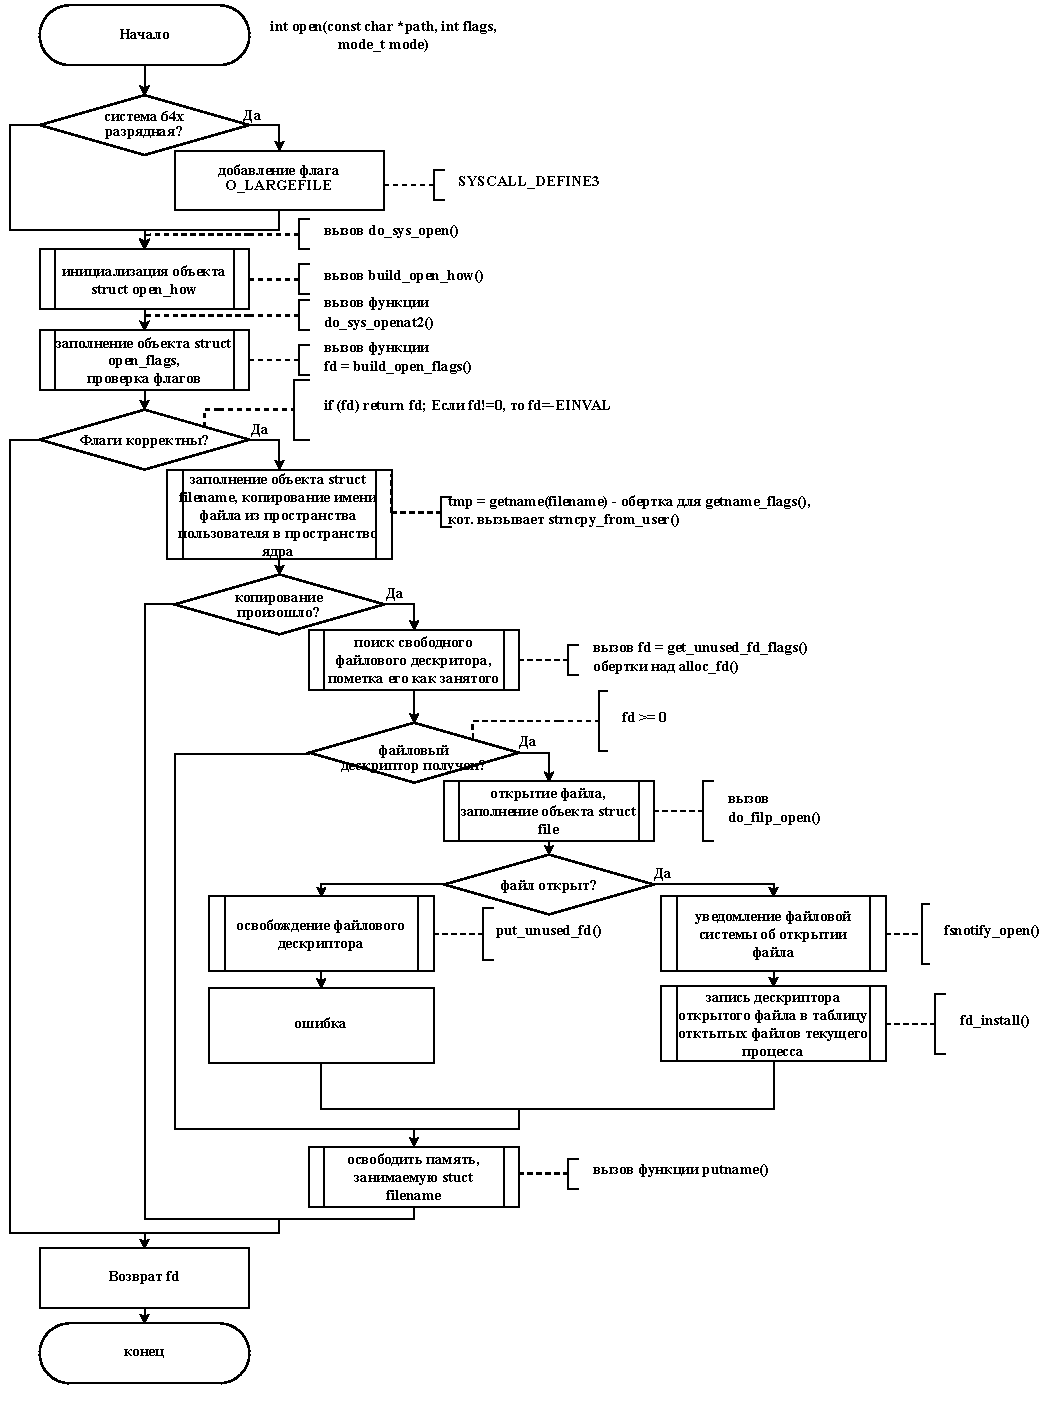
\includegraphics[width=0.8\textwidth]{img/main.pdf}
	\caption{SYSCALL\_DEFINE3}
\end{figure}

\begin{figure}[ht]
	\centering
	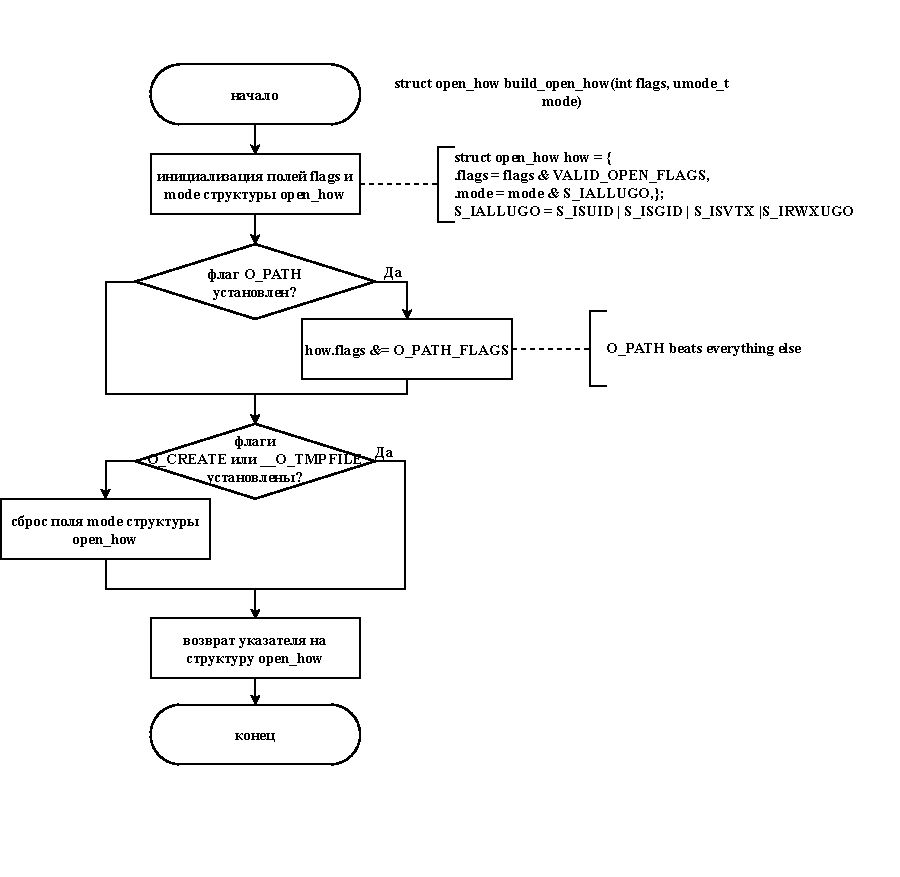
\includegraphics[width=\textwidth]{img/build_open_how.pdf}
	\caption{build\_open\_how()}
\end{figure}

\begin{figure}[ht]
	\centering
	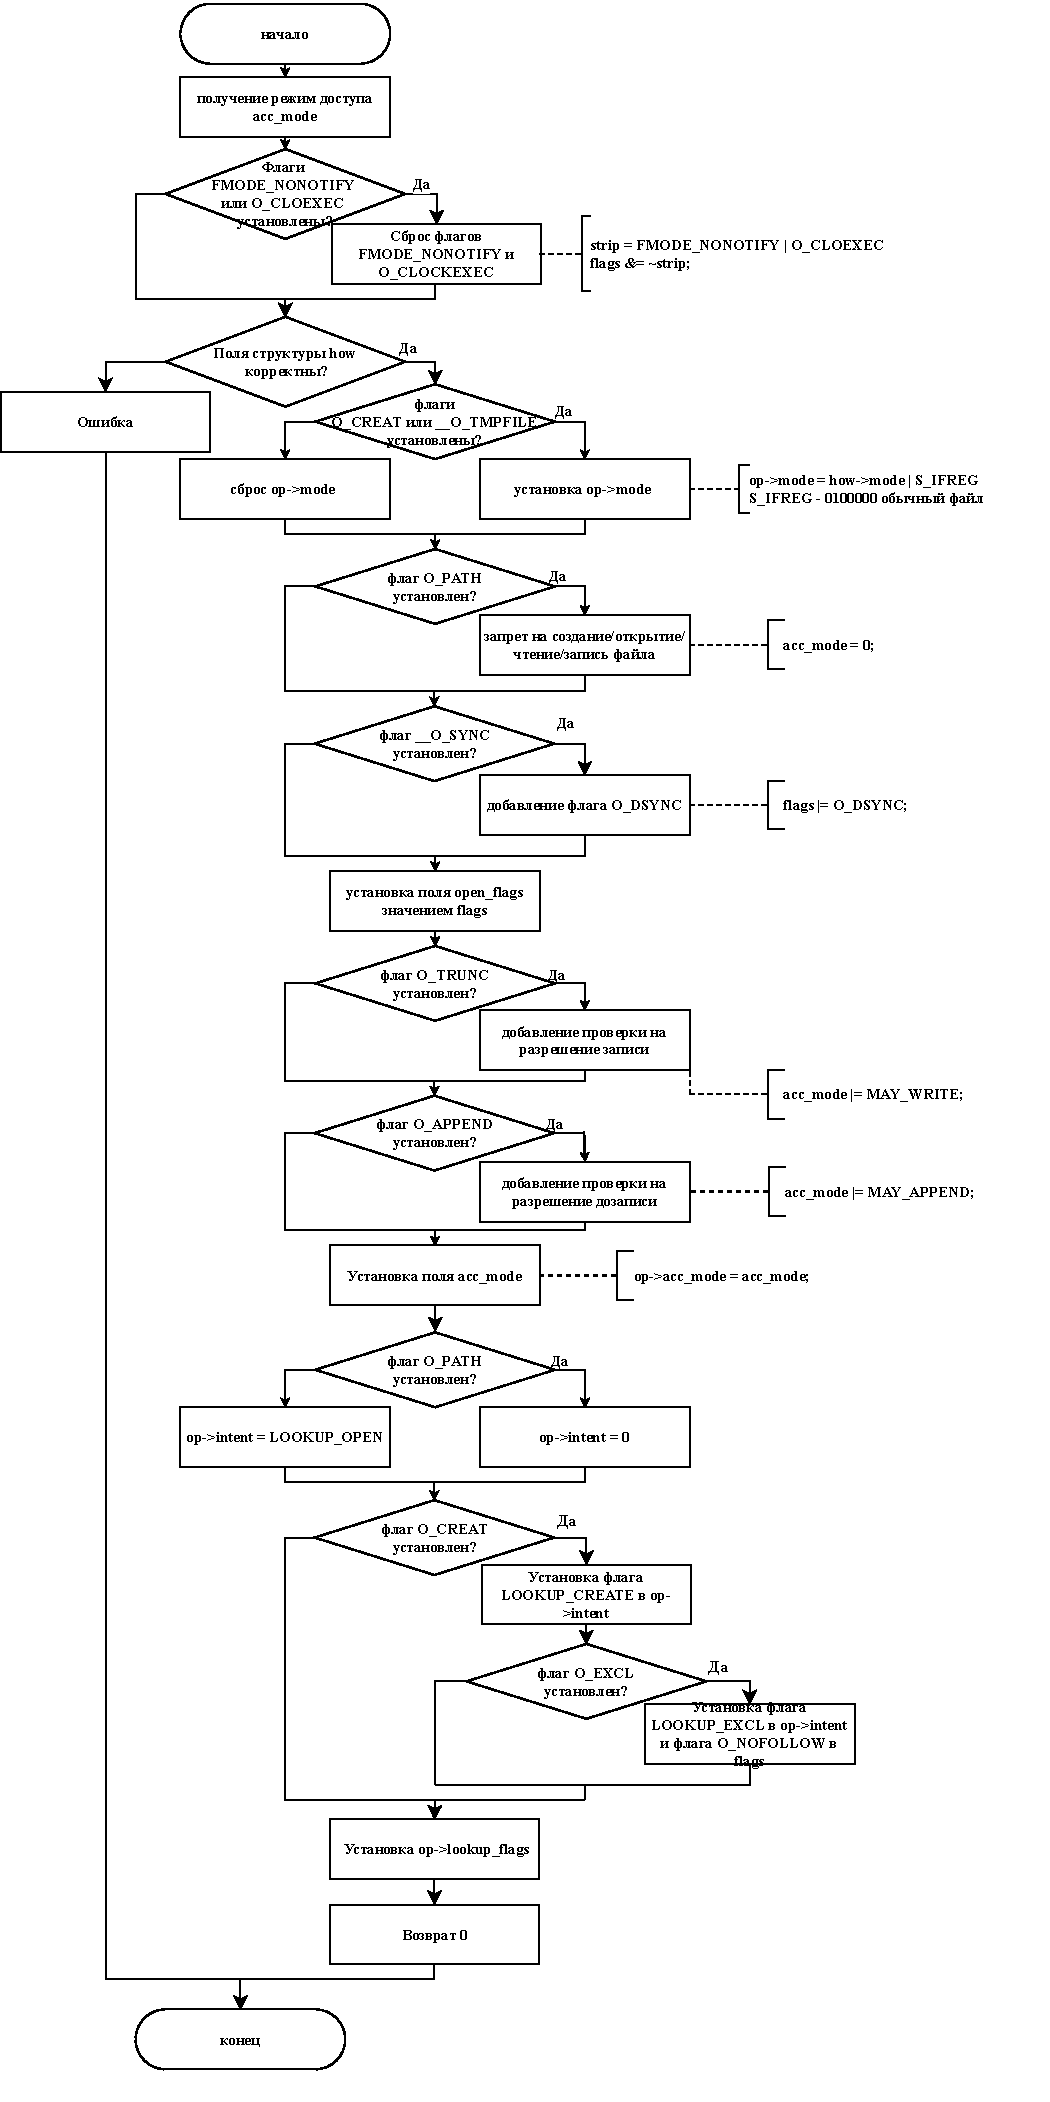
\includegraphics[scale=0.7]{img/build_open_flags.pdf}
	\caption{build\_open\_flags()}
\end{figure}

\begin{figure}[ht]
	\centering
	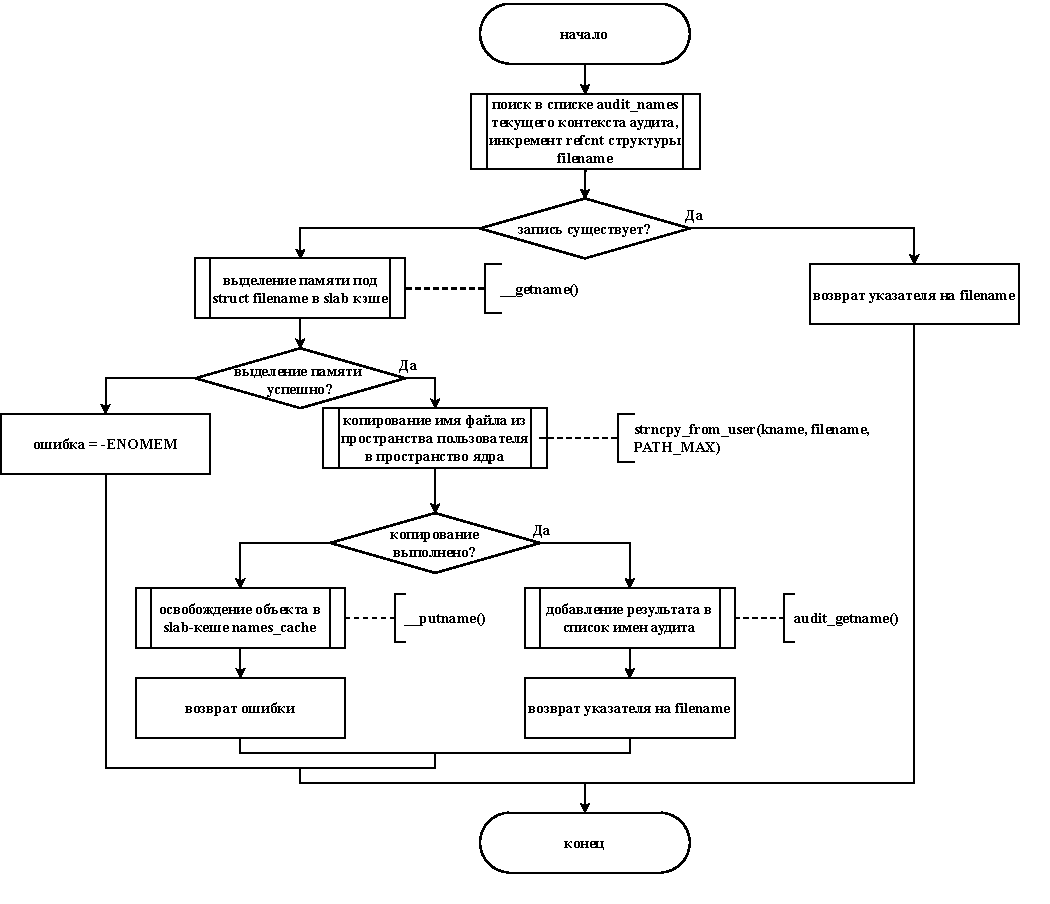
\includegraphics[width=\textwidth]{img/getname_flags.pdf}
	\caption{getname\_flags()}
\end{figure}

\begin{figure}[ht]
	\centering
	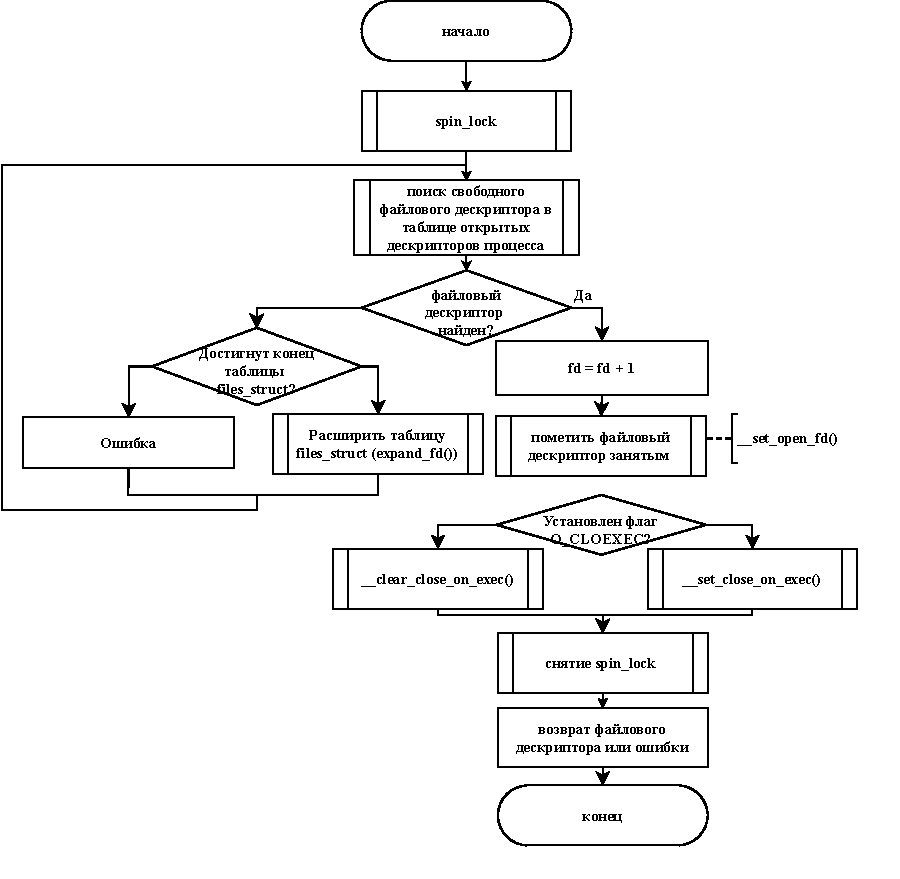
\includegraphics[width=\textwidth]{img/alloc_fd.pdf}
	\caption{alloc\_fd()}
\end{figure}

\clearpage

\begin{figure}[ht]
	\centering
	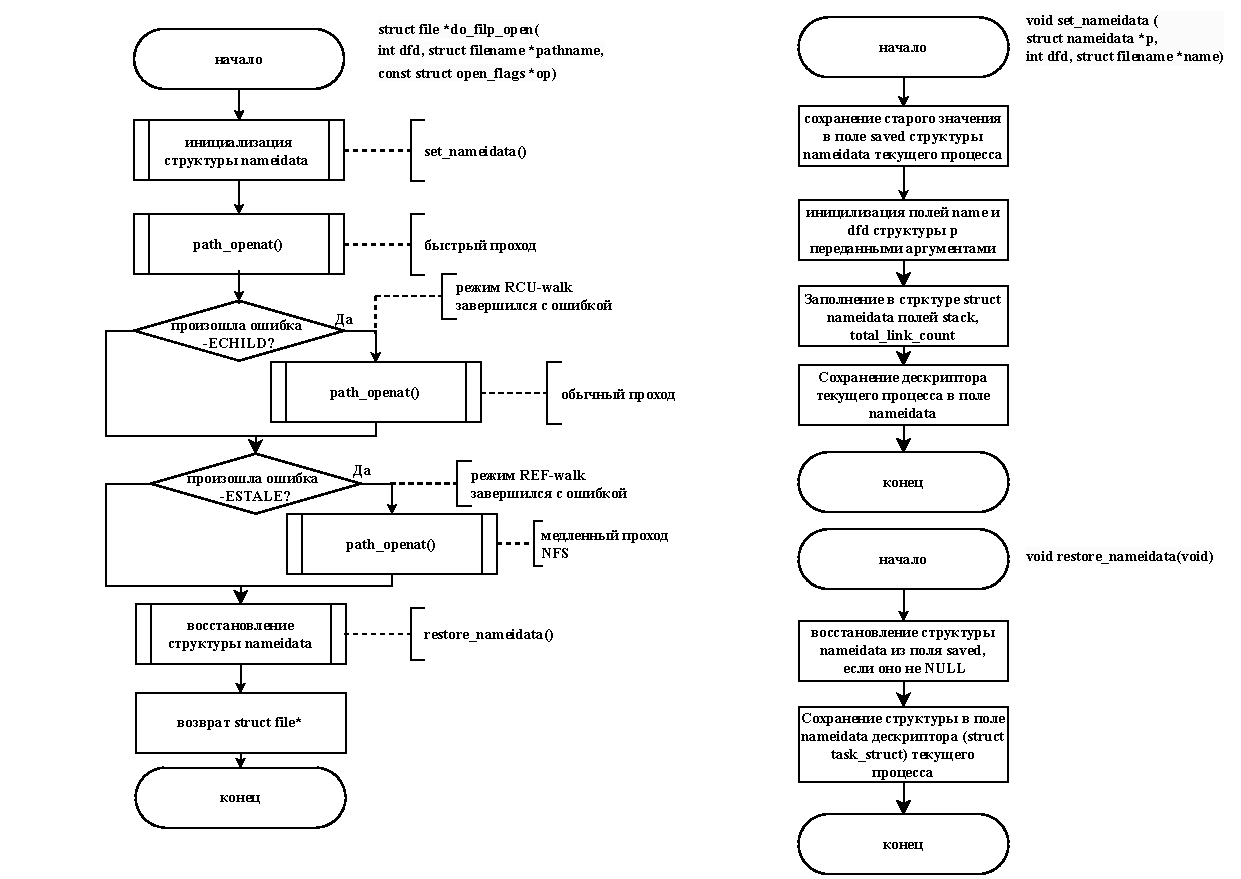
\includegraphics[width=\textwidth]{img/do_filp_open.pdf}
	\caption{do\_filp\_open()}
\end{figure}

\texttt{LOOKUP\_RCU} --- флаг используется в VFS для указания, что операция должна выполняться с использованием RCU (Read-Copy-Update).

\texttt{LOOKUP\_REVAL} --- флаг для работы с NFS, указывает, что необходимо выполнить повторную проверку.

\texttt{O\_APPEND} --- может привести к изменению файлов в файловых системах NFS, если несколько процессов одновременно добавляют данные в файл. Это связано с тем, что в NFS не работает флаг \texttt{O\_APPEND}, поэтому доступ к файл осуществляется в монопольном режиме, что невозможно без состояния гонки.

\begin{figure}[ht]
	\centering
	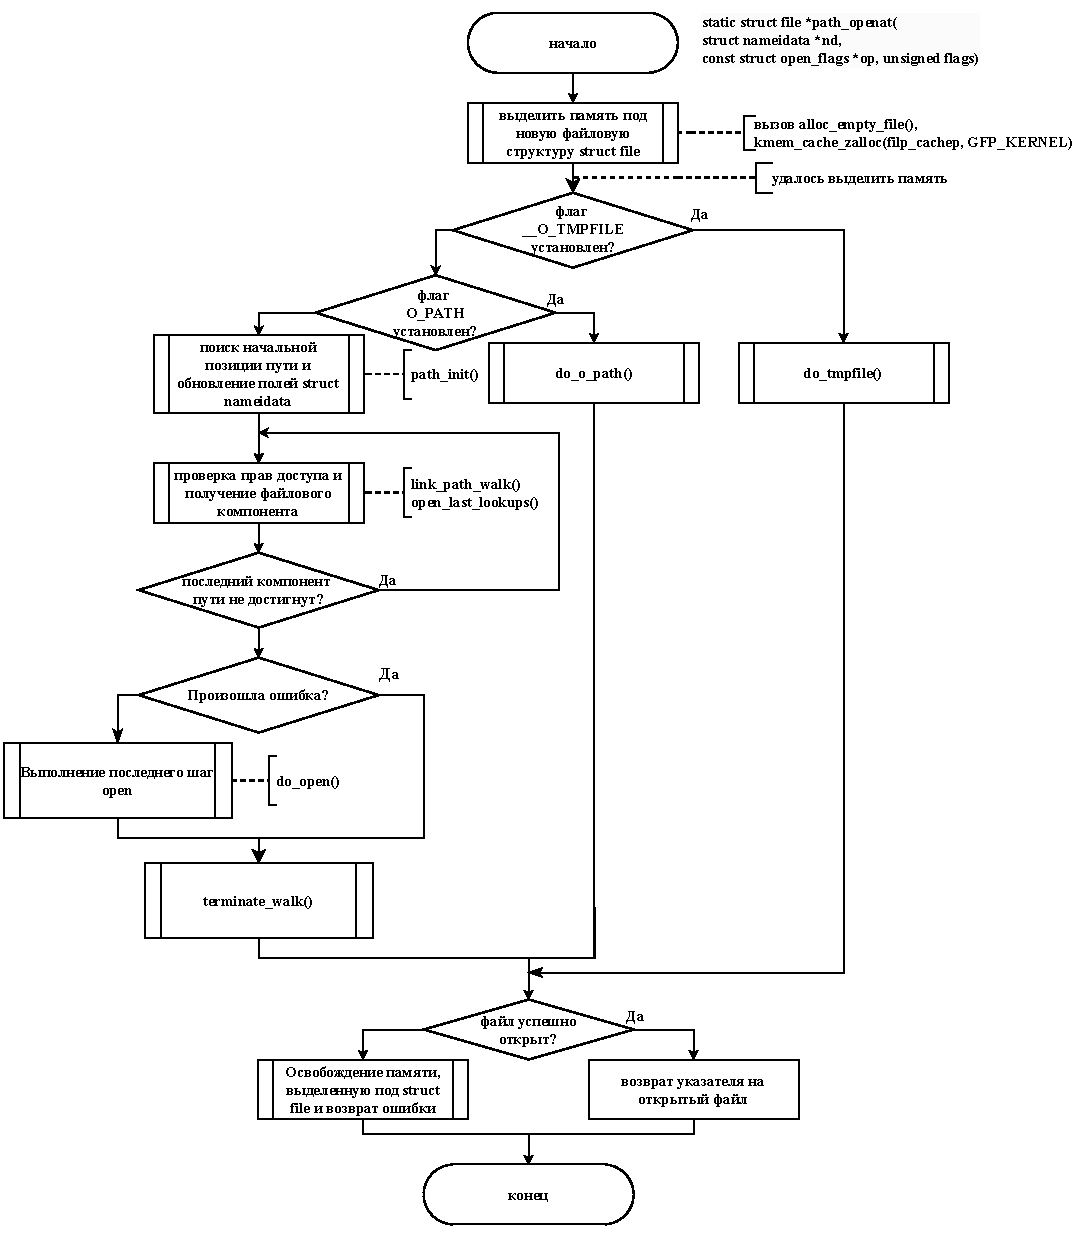
\includegraphics[width=\textwidth]{img/path_openat.pdf}
	\caption{path\_openat()}
\end{figure}

\begin{figure}[ht]
	\centering
	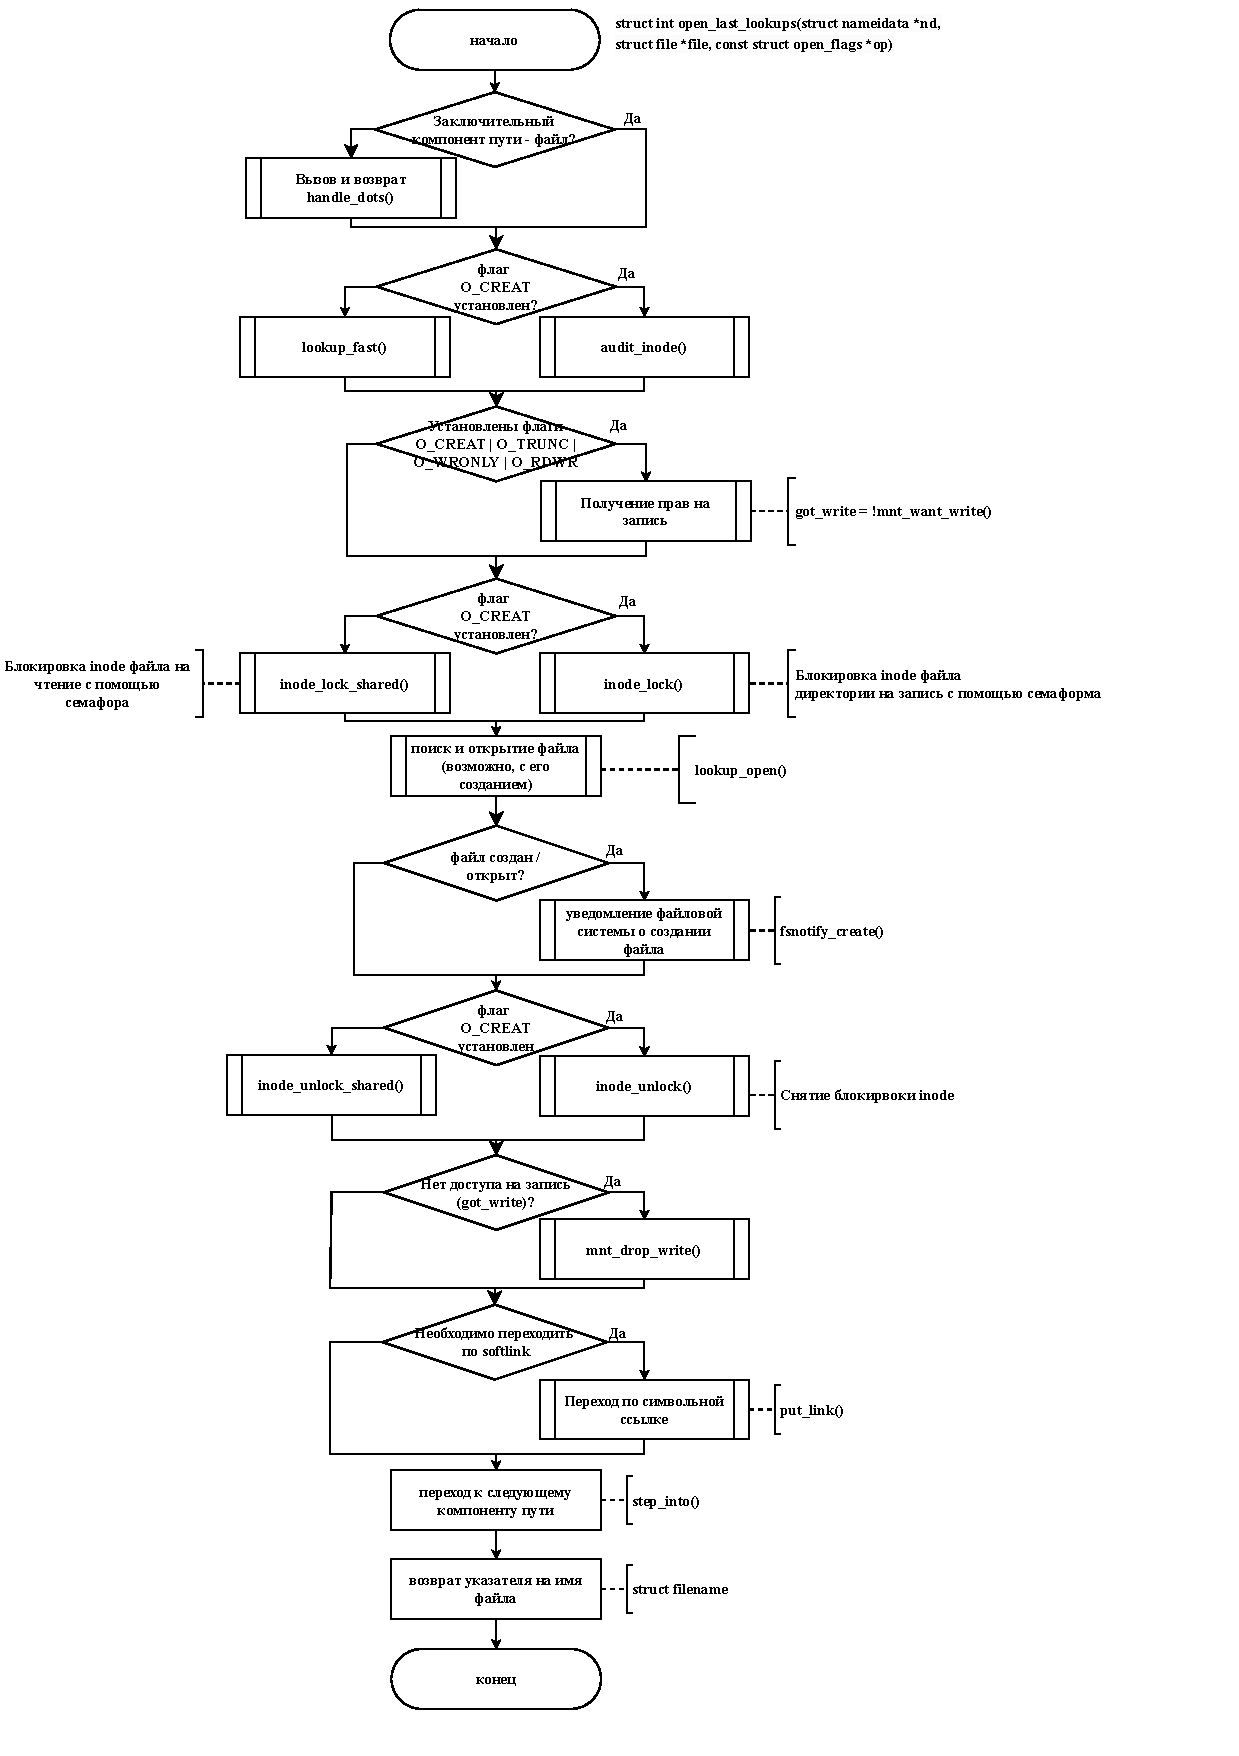
\includegraphics[width=\textwidth]{img/open_last_lookups.pdf}
	\caption{open\_last\_lookups()}
\end{figure}

\begin{figure}[ht]
	\centering
	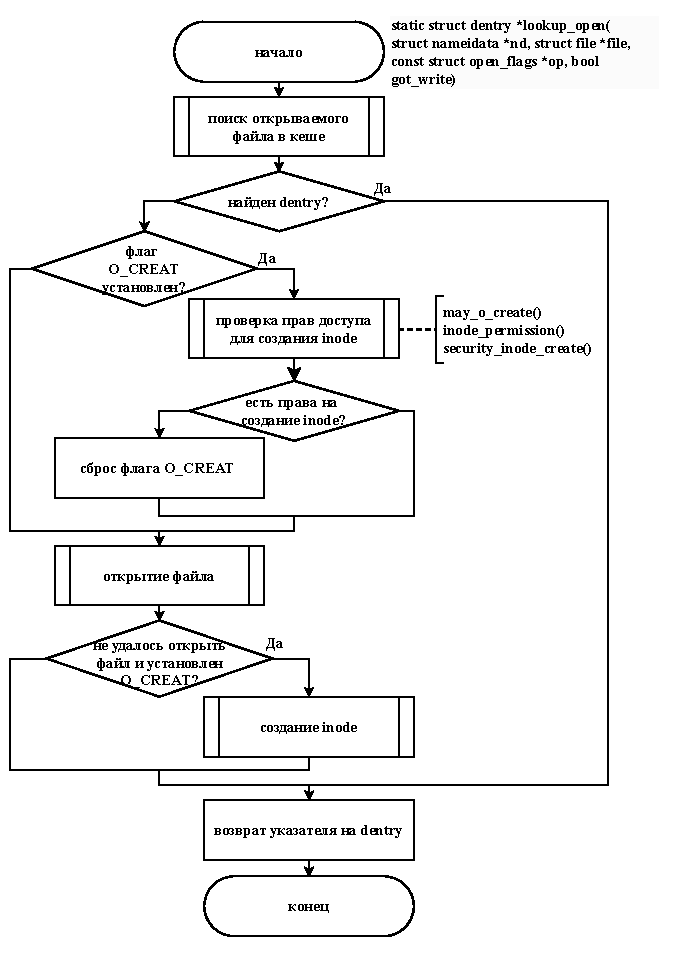
\includegraphics[width=\textwidth]{img/lookup_open.pdf}
	\caption{lookup\_open()}
\end{figure}

\begin{figure}[ht]
	\centering
	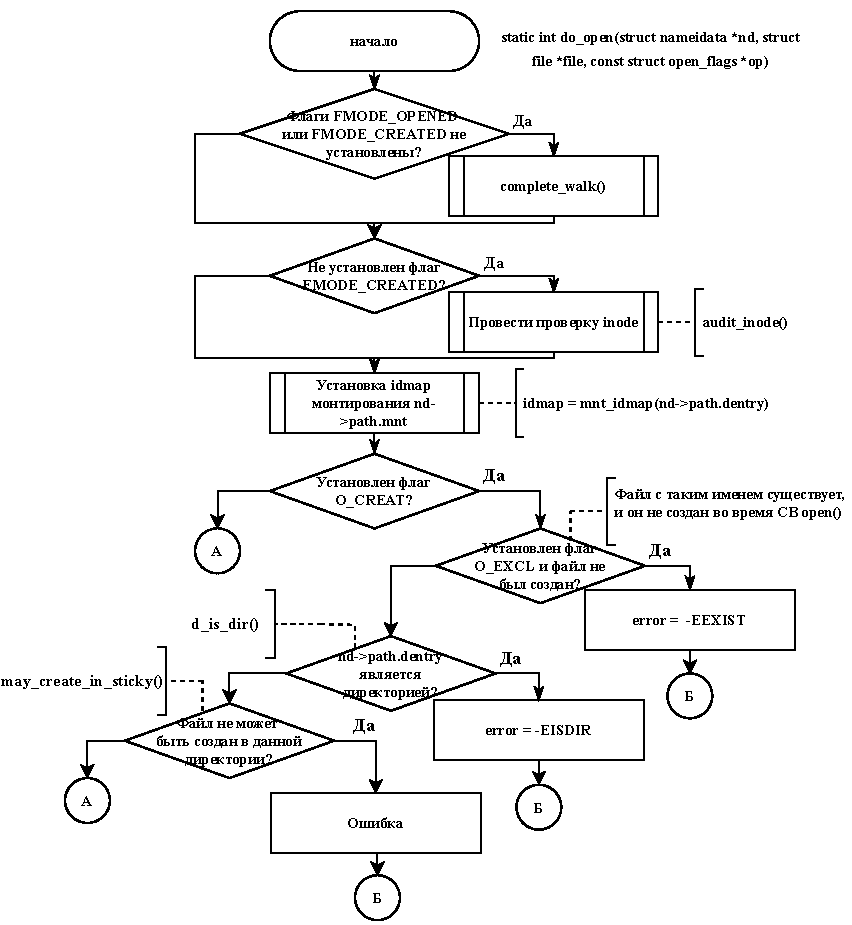
\includegraphics[width=\textwidth]{img/do_open.pdf}
	\caption{do\_open()}
\end{figure}

\begin{figure}[ht]
	\centering
	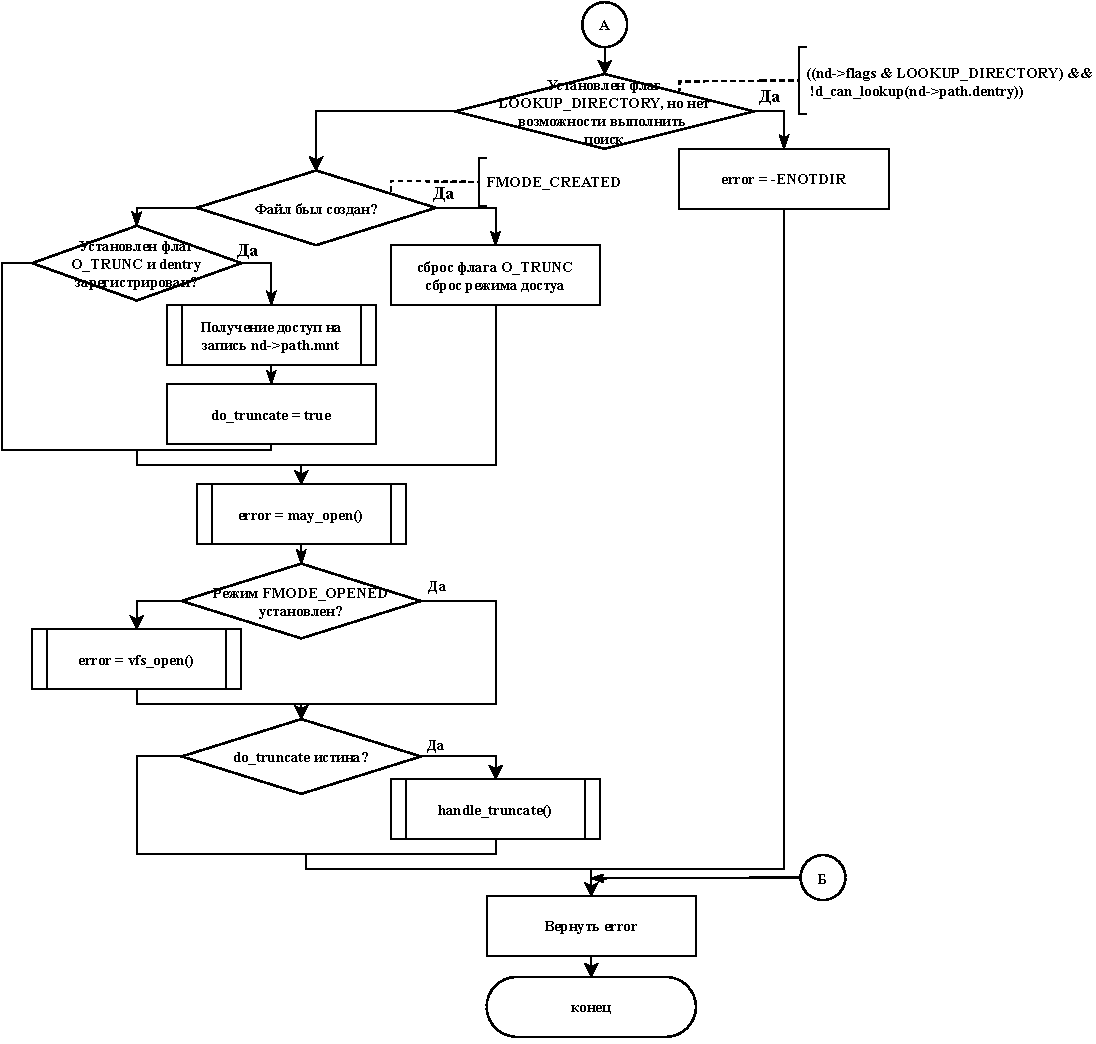
\includegraphics[width=\textwidth]{img/do_open2.pdf}
	\caption{do\_open()}
\end{figure}
